\documentclass[a4paper,12pt]{article}
\usepackage[utf8x]{inputenc}
\usepackage{graphicx}
\usepackage{euler}
\usepackage{palatino}
\usepackage{listings}
\usepackage{tikz} 
%opening
\title{Tutorial 1. Introduction to MOA \\ \{M\}assive \{O\}nline \{A\}nalysis}
\author{Albert Bifet and Richard Kirkby}
\date{March 2012}

\newtheorem{definition}{Definition}{}
\newtheorem{exercise}{Exercise}{}

\begin{document}
\lstset{language=Java,basicstyle=\tiny,numbers=left}
\maketitle
\begin{center}

\includegraphics[height=3cm]{figures/LogoMOA.jpg} \\

\includegraphics[height=4cm]{figures/Waikato.jpg} \\ 
\end{center}
\thispagestyle{empty}
\newpage
\setcounter{page}{1}

\section{Getting Started}

This tutorial is a basic introduction to MOA.
{\bf M}assive {\bf O}nline {\bf A}nalysis (MOA) is a  
software environment for implementing algorithms and running experiments
for online learning from 
evolving data streams.

We suppose that MOA is installed in your system.
Start a graphical user interface for configuring and running tasks with the command:

\begin{verbatim}
java -cp moa.jar -javaagent:sizeofag.jar moa.gui.GUI
\end{verbatim}

\begin{figure}[h]
\begin{center} 
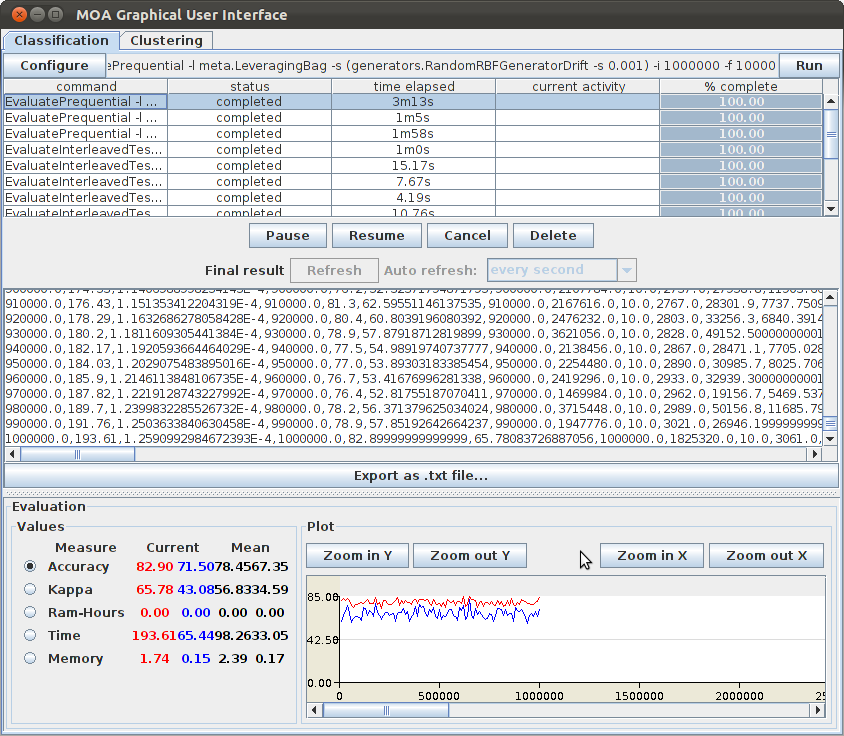
\includegraphics[height=2.5in]{figures/MOA_Task.png}
\end{center} 
\caption{MOA Graphical User Interface}
\label{fig:moagui}
\end{figure}

Click 'Configure' to set up a task, when ready click to launch a task click 'Run'. Several tasks can be run concurrently. 
Click on different tasks in the list and control them using the buttons below.
 If textual output of a task is available it will be displayed in the middle of the GUI, and can be saved to disk.

Note that the command line text box displayed at the top of the window represents textual commands that can be used to run tasks on the command line.
 The text can be selected then copied onto the clipboard. In the bottom of the GUI there is a graphical display of the results. It is possible
to compare the results of two different tasks: the current task is displayed in red, and the selected previously is in blue. 

\section{The Classification Graphical User Interface}

We start comparing the accuracy of two classifiers. First, we explain briefly two different data stream evaluations.% have to decide which data stream evaluation to use.

\subsection{Data streams Evaluation}
The most significant requirements for a data stream setting are the following: 
\begin{description}
\item[Requirement 1] Process an example at a time, and inspect
 it only once (at most)
\item[Requirement 2] Use a limited amount of memory
\item[Requirement 3] Work in a limited amount of time
\item[Requirement 4] Be ready to predict at any time
\end{description}
\begin{figure}[t]
\begin{center} 
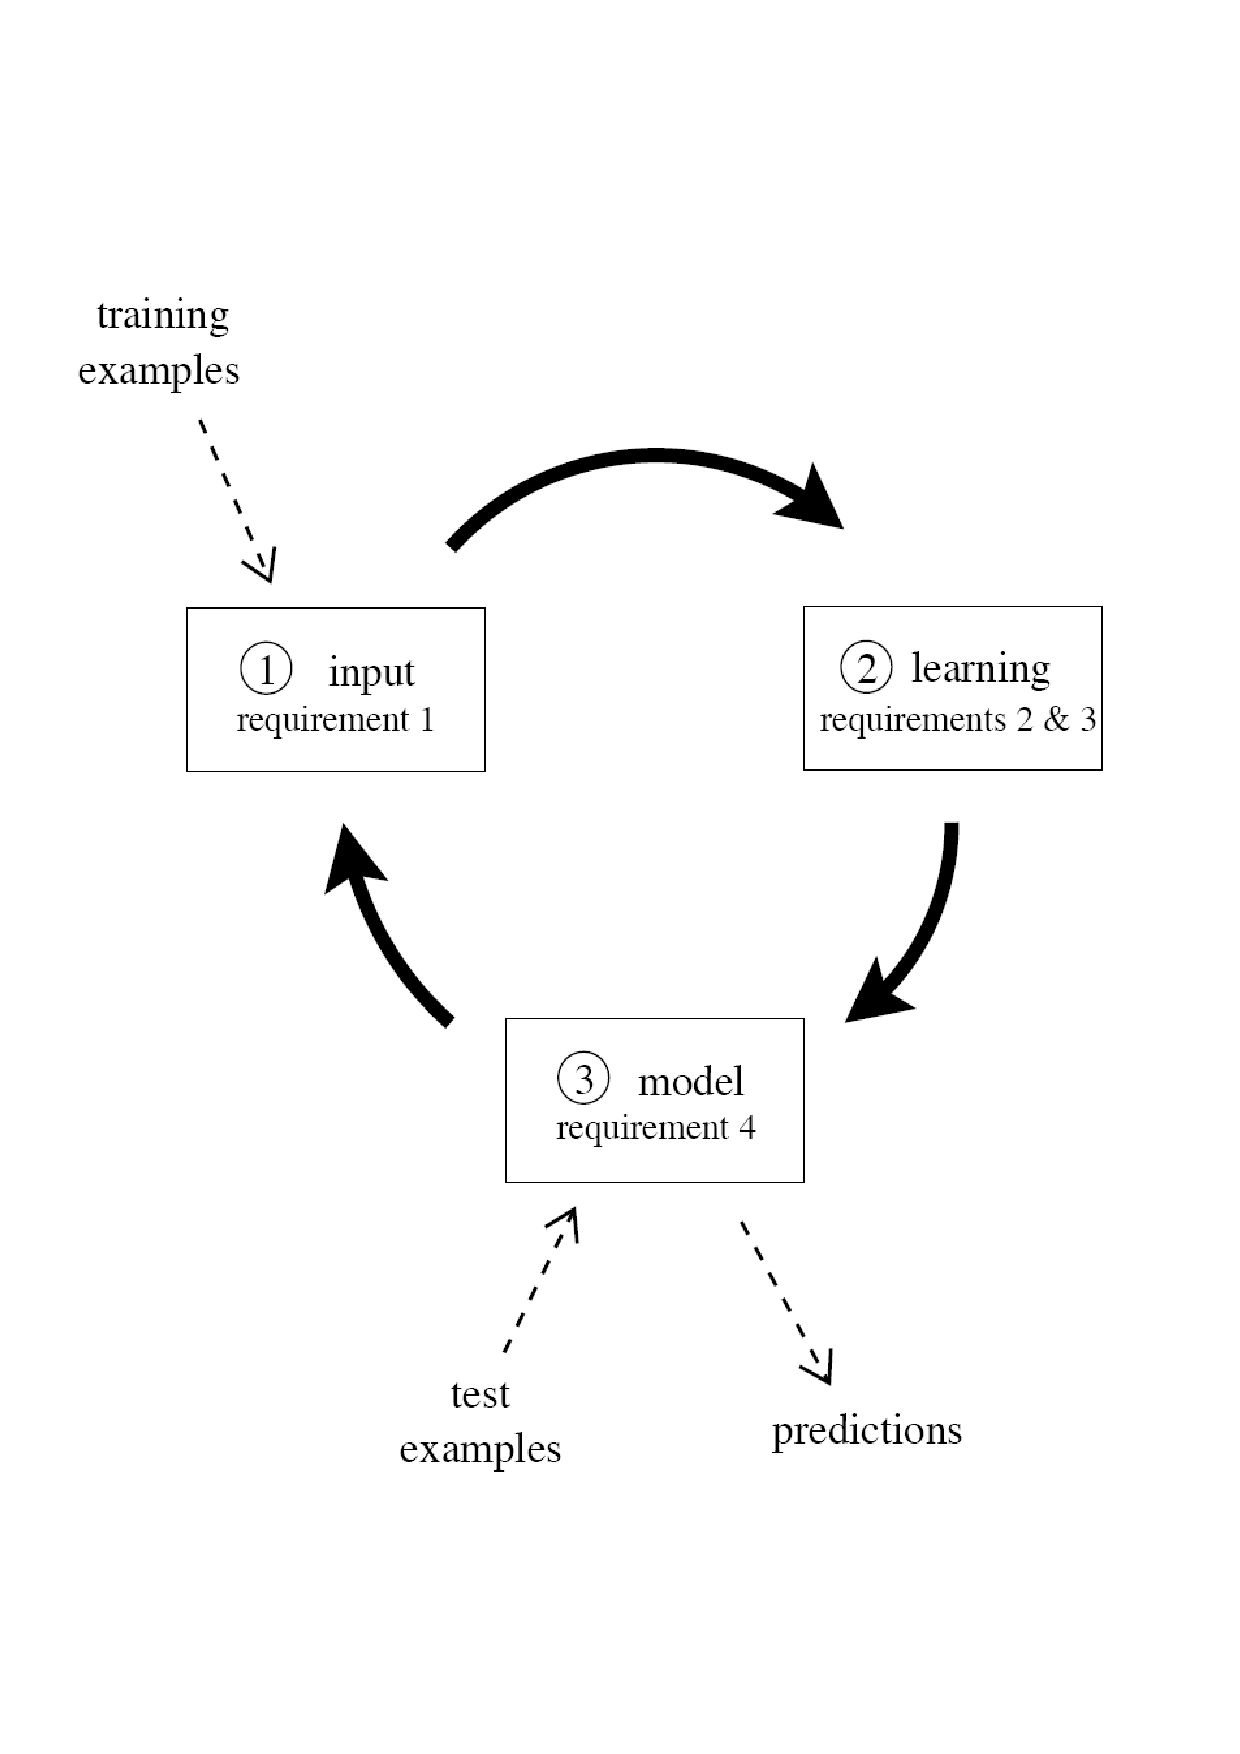
\includegraphics[height=9cm]{figures/Frame.pdf}
\end{center} 
\caption{The data stream classification cycle}
\label{fig:cycle}
\end{figure} 

Figure~\ref{fig:cycle} illustrates the typical use of a data stream 
classification algorithm, and how the requirements fit 
in a repeating cycle:
\begin{enumerate}
\item  The algorithm is passed the next available example from the stream
   (requirement 1).
\item  The algorithm processes the example, updating its data structures. It
   does so without exceeding the memory bounds set on it (requirement 2),
   and as quickly as possible (requirement 3).
\item  The algorithm is ready to accept the next example. On request it is
   able to predict the class of unseen examples
   (requirement 4).
\end{enumerate}

In traditional batch learning the problem of limited data is overcome
by analyzing and averaging multiple models produced with different random
arrangements of training and test data. In the stream setting the problem of
(effectively) unlimited data poses different challenges. One solution involves
taking snapshots at different times during the induction of a model to see how
much the model improves.

    When considering what procedure to use in the data stream setting, one of
the unique concerns is how to build a picture of accuracy over time. Two main
approaches arise:
\begin{itemize}
 \item {\bf Holdout}:
When traditional batch learning reaches a scale where cross-validation is too time 
consuming, it is often accepted to instead measure performance on a single holdout
set. This is most useful when the division between train and test sets have
been pre-defined, so that results from different studies can be directly compared. 
\item {\bf Interleaved Test-Then-Train or Prequential}:
 Each individual example can be used to test the model
before it is used for training, and from this the accuracy can be incrementally
updated. When intentionally performed in this order, the model is always
being tested on examples it has not seen. This scheme has the advantage that
no holdout set is needed for testing, making maximum use of the available
data. It also ensures a smooth plot of accuracy over time, as each individual
example will become increasingly less significant to the overall average.
\end{itemize}
   
Holdout evaluation gives a more accurate estimation of the accuracy of the classifier on more recent data. However, it requires recent test data that it is difficult to obtain for real datasets.
Gama et al. 
propose to use a forgetting mechanism for estimating holdout accuracy using
prequential
accuracy: a sliding window of size $w$ with the most recent
observations, or fading factors that weigh observations using a decay
factor $\alpha$. 
The output of the two mechanisms is very
similar (every window of size $w_0$ may be approximated by some decay
factor $\alpha_0$).

As data stream classification is a relatively new field, such evaluation 
practices are not nearly as well researched and established as they are
in the traditional batch setting. 


\subsection{Exercises}

To familiarize yourself with the functions discussed so far, please do the following
two exercises. The solutions to these and other exercises in this tutorial are given
at the end.

\begin{exercise}
Compare the accuracy of the Hoeffding Tree with the Naive Bayes classifier, for a RandomTreeGenerator stream of 1,000,000 instances using Interleaved Test-Then-Train evaluation.
Use for all exercises a sample frequency of $10,000$.
\end{exercise}
\begin{exercise}
Compare and discuss the accuracy for the same stream of the previous exercise using three different evaluations with a Hoeffding Tree:
\begin{itemize}
 \item Periodic Held Out with 1,000 instances for testing
 \item Interleaved Test Then Train
 \item Prequential with a sliding window of 1,000 instances.
\end{itemize}
\end{exercise}

\subsection{Drift Stream Generators}

MOA streams are build using generators, reading ARFF files, joining several streams, or filtering streams.
MOA streams generators allow to simulate potentially infinite sequence of data.

Two streams evolving on time are:
\begin{itemize}
\item Rotating Hyperplane
\item Random RBF Generator
\end{itemize}

To model concept drift we only have to set up the drift parameter of the stream. 

We can model concept drift also joining several streams.
MOA models
a concept drift {event} as a weighted combination
of two pure distributions that characterizes the target concepts before and after
the drift.  MOA uses 
the sigmoid function, as an elegant and practical solution to define the probability that every new 
instance of the stream belongs to the new concept after the drift.

\begin{figure}
\begin{tikzpicture}[domain=-2:9]
  \draw[step=2,very thin,color=gray] (-0.1,-0.1) grid (8.2,4.2);
  \draw[->] (-2.2,0) -- (8.2,0) node[right] {$t$};
  \draw[->] (0,-0.2) -- (0,4.2) node[above] {$f(t)$};
  \draw[<->] (2,-0.6) -- (6,-0.6) node[below] {};
  \draw[color=blue!50!black, domain=2:6] plot[id=x]   function{(x-2)}           node[right]{}; %{$f(x) =x$};
  \draw[color=red!50!black] plot[id=exp] function{4/(1+exp(4-x))} node[right] {$f(t)$};% = 1/{(1+ \mathrm e^{-s (x-x_0)}})$};
  \colorlet{anglecolor}{blue!50!black}
  \filldraw[fill=blue!20,draw=anglecolor] (2,0) -- (2.5,0) arc(0:45:.5);
  \draw (2.7,.3) node[anglecolor] {$\alpha$};
  \filldraw[fill=blue!20,draw=anglecolor] (4,2) -- (4.5,2) arc(0:45:.5);
  \draw (4.7,2.3) node[anglecolor] {$\alpha$};

  \draw (4,-0.3) node[] {$t_0$};
  \draw (4,-0.9) node[] {$W$};
  \draw (-0.5,2) node[] {$0.5$};
  \draw (-0.5,4) node[] {$1$};

\end{tikzpicture}
\caption{A sigmoid function $f(t) = 1/{(1+ \mathrm e^{-s (t-t_0)}})$.}
\label{fig:ConceptChange}
\end{figure}

We see from Figure~\ref{fig:ConceptChange} that the sigmoid function 
$$f(t) = 1/{(1+ \mathrm e^{-s (t-t_0)}})$$
has a derivative at the point $t_0$ equal to $f'(t_0) = s/4$. The tangent of angle 
$\alpha$ is equal to this derivative, $\tan \alpha = s/4$. We observe that 
$ \tan \alpha = 1/ W$,
and as $s= 4 \tan \alpha$ then $s=4/W$. So the parameter $s$ in the sigmoid 
gives the length of $W$ and the angle $\alpha$. 
In this sigmoid model we only need to specify two parameters : 
$t_0$ the point of change, and $W$ the length of change.
Note that for any positive real number $\beta$ $$f(t_0+\beta \cdot W)=1 -f(t_0-\beta \cdot W),$$ and  that $f(t_0+\beta \cdot W)$ and $f(t_0-\beta \cdot W)$ 
are constant values that don't depend on $t_0$ and $W$: 
$$f(t_0+W/2) = 1 - f(t_0-W/2) = 1/( 1+ e^{-2}) \approx 88.08 \%$$  
$$f(t_0+W) = 1 - f(t_0-W) = 1/( 1+ e^{-4}) \approx 98.20 \%$$  
$$f(t_0+2W) = 1 - f(t_0-2W) = 1/( 1+ e^{-8}) \approx 99.97 \%$$

\begin{definition} %{\bf ($\oplus$-operation)}\\
Given two data streams $a$, $b$, we define $c = a  \oplus^{W}_{t_0} b$ as the 
data stream built joining the two data streams $a$ and $b$, where
$t_0$ is the point of change, $W$ is the length of change and 
\begin{itemize}
 \item $\Pr[ c(t) = a(t)] = \mathrm e^{-4(t-t_0)/W}/{(1+ \mathrm e^{-4(t-t_0)/W})}$
 \item $\Pr[ c(t) = b(t)] = 1/{(1+ \mathrm e^{-4(t-t_0)/W})}$.
\end{itemize}
\end{definition}


Example:
\begin{footnotesize}\begin{verbatim}
 ConceptDriftStream -s (generators.AgrawalGenerator -f 7) 
    -d (generators.AgrawalGenerator -f 2) -w 1000000 -p 900000 
\end{verbatim}\end{footnotesize}
\texttt{ConceptDriftStream} parameters:

\begin{itemize}
\item -s : Stream 
\item -d : Concept drift Stream
\item -p : Central position of concept drift change
\item -w : Width of concept drift change\end{itemize}


\subsection{Exercises}

\begin{exercise}Compare the accuracy of the Hoeffding Tree with the Naive Bayes classifier, for a RandomRBFGenerator stream of 1,000,000 instances with speed change of 0,001 using Interleaved Test-Then-Train evaluation.  
\end{exercise}
\begin{exercise}Compare the accuracy for the same stream of the previous exercise using three different classifiers:
\begin{itemize}
 \item Hoeffding Tree with Majority Class at the leaves
 \item Hoeffding Adaptive Tree
 \item OzaBagAdwin with 10 HoeffdingTree

\end{itemize}
\end{exercise}


\section{Using the command line}

An easy way to use the command line, is to copy and paste the text in the Configuration line of the Graphical User Interface.% at the end of

For example, suppose we want to process the task 
\begin{verbatim}EvaluatePrequential -l trees.HoeffdingTree -i 1000000 -w 10000\end{verbatim} 
using the command line. We simply write 
\begin{verbatim}
java -cp moa.jar -javaagent:sizeofag.jar moa.DoTask  \
"EvaluatePrequential -l trees.HoeffdingTree -i 1000000 -w 10000"
\end{verbatim}

Note that some parameters are missing, since they use default values.


\subsection{Learning and Evaluating Models}

The \verb+moa.DoTask+ class is the main class for running tasks on the command line. It will accept the name of a task followed by any appropriate parameters. The first task used is the \verb+LearnModel+ task. The \verb+-l+ parameter specifies the learner, in this case the \verb+HoeffdingTree+ class. The \verb+-s+ parameter specifies the stream to learn from, in this case {\tt generators.Wave- formGenerator} is specified, which is a data stream generator that produces a three-class learning problem of identifying three types of waveform. The \verb+-m+ option specifies the maximum number of examples to train the learner with, in this case one million examples. The \verb+-O+ option specifies a file to output the resulting model to:

\begin{verbatim}
java -cp moa.jar -javaagent:sizeofag.jar moa.DoTask \
  LearnModel -l trees.HoeffdingTree \
  -s generators.WaveformGenerator -m 1000000 -O model1.moa
\end{verbatim}

This will create a file named \verb+model1.moa+ that contains the decision stump model that was induced during training.

The next example will evaluate the model to see how accurate it is on a set of examples that are generated using a different random seed. The \verb+EvaluateModel+ task is given the parameters needed to load the model produced in the previous step, generate a new waveform stream with a random seed of 2, and test on one million examples:

\begin{verbatim}
java -cp moa.jar -javaagent:sizeofag.jar moa.DoTask \
  "EvaluateModel -m file:model1.moa \
  -s (generators.WaveformGenerator -i 2) -i 1000000"
\end{verbatim}

This is the first example of nesting parameters using brackets. Quotes have been added around the description of the task, otherwise the operating system may be confused about the meaning of the brackets.

After evaluation the following statistics are output:

\begin{verbatim}
classified instances = 1,000,000
classifications correct (percent) = 84.474
Kappa Statistic (percent) = 76.711
\end{verbatim}

Note the the above two steps can be achieved by rolling them into one, avoiding the need to create an external file, as follows:

\begin{verbatim}
java -cp moa.jar -javaagent:sizeofag.jar moa.DoTask \
  "EvaluateModel -m (LearnModel -l trees.HoeffdingTree \
  -s generators.WaveformGenerator -m 1000000) \
  -s (generators.WaveformGenerator -i 2) -i 1000000"
\end{verbatim}

The task \verb+EvaluatePeriodicHeldOutTest+ will train a model while taking snapshots of performance using a held-out test set at periodic intervals.
The following command creates a {\em comma separated values} file, training the \verb+HoeffdingTree+ classifier on the \verb+WaveformGenerator+ data, using the first 100 thousand examples for testing, training on a total of 100 million examples, and testing every one million examples:

\begin{verbatim}
java -cp moa.jar -javaagent:sizeofag.jar moa.DoTask \
  "EvaluatePeriodicHeldOutTest -l trees.HoeffdingTree \
  -s generators.WaveformGenerator \
  -n 100000 -i 10000000 -f 1000000" > dsresult.csv
\end{verbatim}

\subsection{Exercises}
\begin{exercise}
Repeat the experiments of exercises 1 and 2 using the command line.  
\end{exercise}

\begin{exercise}
Compare accuracy and RAM-Hours needed using a prequential evaluation (sliding window of 1,000 instances) of 1,000,000 instances for a Random Radius Based Function stream with speed of change 0,001 using the following methods:
\begin{itemize}
 \item OzaBag with 10 HoeffdingTree
 \item OzaBagAdwin with 10 HoeffdingTree
 \item LeveragingBag with 10 HoeffdingTree
\end{itemize}
\end{exercise}

\section{Answers To Exercises}

\begin{enumerate}
 \item Naive Bayes: $73.63\%$ Hoeffding Tree : $ 94.45\%$
 \item \begin{itemize}
        \item Periodic Held Out with 1,000 instances for testing :$96.5\%$
	\item Interleaved Test Then Train : $ 94.45\%$
	\item Prequential with a sliding window of 1,000 instances: $96.7\%$.
       \end{itemize}
\item Naive Bayes: $53.14\%$ Hoeffding Tree : $57.60\%$
\item \begin{itemize}
       \item Hoeffding Tree with Majority Class at Leaves: $51.71\%$
       \item Hoeffding Adaptive Tree: $65.28\%$
	\item OzaBagAdwin with 10 HoeffdingTree: $67.23\%$
      \end{itemize}
\item \begin{itemize}
        \item \texttt{EvaluateInterleavedTestThenTrain -i 1000000}
	\item \texttt{EvaluateInterleavedTestThenTrain -l trees.HoeffdingTree -i 1000000}
	\item \texttt{EvaluatePeriodicHeldOutTest -n 1000 -i 1000000}
	\item \texttt{EvaluateInterleavedTestThenTrain -l trees.HoeffdingTree -i 1000000}
	\item \texttt{EvaluatePrequential -l trees.HoeffdingTree -i 1000000}
       \end{itemize}
\item \begin{itemize}
 \item
 OzaBag with 10 HoeffdingTree:
\begin{itemize} \item  
$57.4\%$ Accuracy, $4 \cdot 10^{-4}$ RAM-Hours
\end{itemize}
 \item
 OzaBagAdwin with 10 HoeffdingTree: 
\begin{itemize} \item  
$71.5\%$ Accuracy, $2.93 \cdot 10^{-6}$ RAM-Hours
\end{itemize}
 \item
 LeveragingBag with 10 HoeffdingTree:
\begin{itemize} \item 
 $82.9\%$ Accuracy, $1.25 \cdot 10^{-4}$  RAM-Hours 
 \end{itemize}
\end{itemize}

\end{enumerate}

\end{document}
